\documentclass[10pt,a4paper,]{article}

%% %%%%%%%%%%%%%%%%%%%%%%%%%%%%%%%%%%%%%%%%%%%%%%%%%%%%%%%%%%%%%%%%%%%%%%%%%%%%%%%%%%%%%%
%%
%%   BScBI_CompGenomics_template.tex
%%
%%   A LaTeX template for MarkDown reports to submit as BScBI-CG practical exercises.
%%
%% %%%%%%%%%%%%%%%%%%%%%%%%%%%%%%%%%%%%%%%%%%%%%%%%%%%%%%%%%%%%%%%%%%%%%%%%%%%%%%%%%%%%%%
%%
%%                 CopyLeft 2020 (CC:BY-NC-SA) --- Josep F Abril
%%
%%   This file should be considered under the Creative Commons BY-NC-SA License
%%   (Attribution-Noncommercial-ShareAlike). The material is provided "AS IS", 
%%   mainly for teaching purposes, and is distributed in the hope that it will
%%   be useful, but WITHOUT ANY WARRANTY; without even the implied warranty
%%   of MERCHANTABILITY or FITNESS FOR A PARTICULAR PURPOSE.
%%
%% %%%%%%%%%%%%%%%%%%%%%%%%%%%%%%%%%%%%%%%%%%%%%%%%%%%%%%%%%%%%%%%%%%%%%%%%%%%%%%%%%%%%%%

\usepackage[pdftex]{graphicx}
\usepackage{xcolor} %%% FIX %%%
\usepackage{fancyvrb}
\usepackage{comment}
\usepackage{fancyhdr} % Do not use \usepackage{fancybox} -> TOCs disappear
\usepackage{multirow}
\usepackage[nottoc,notlof,notlot,numbib]{tocbibind}

\usepackage{lmodern}
\usepackage{amssymb,amsmath}
\usepackage{ifxetex,ifluatex}
\usepackage{fixltx2e} % provides \textsubscript
\ifnum 0\ifxetex 1\fi\ifluatex 1\fi=0 % if pdftex
  \usepackage[T1]{fontenc}
  \usepackage[utf8]{inputenc}
\else % if luatex or xelatex
  \ifxetex
    \usepackage{mathspec}
    \usepackage{xltxtra,xunicode}
  \else
    \usepackage{fontspec}
  \fi
  \defaultfontfeatures{Mapping=tex-text,Scale=MatchLowercase}
  \newcommand{\euro}{€}
\fi
% use upquote if available, for straight quotes in verbatim environments
\IfFileExists{upquote.sty}{\usepackage{upquote}}{}
% use microtype if available
\IfFileExists{microtype.sty}{%
\usepackage{microtype}
\UseMicrotypeSet[protrusion]{basicmath} % disable protrusion for tt fonts
}{}
\usepackage[margin=1.5cm]{geometry}
\usepackage{natbib}
\bibliographystyle{plainnat}
\usepackage{color}
\usepackage{fancyvrb}
\newcommand{\VerbBar}{|}
\newcommand{\VERB}{\Verb[commandchars=\\\{\}]}
\DefineVerbatimEnvironment{Highlighting}{Verbatim}{commandchars=\\\{\}}
% Add ',fontsize=\small' for more characters per line
\newenvironment{Shaded}{}{}
\newcommand{\AlertTok}[1]{\textcolor[rgb]{1.00,0.00,0.00}{\textbf{#1}}}
\newcommand{\AnnotationTok}[1]{\textcolor[rgb]{0.38,0.63,0.69}{\textbf{\textit{#1}}}}
\newcommand{\AttributeTok}[1]{\textcolor[rgb]{0.49,0.56,0.16}{#1}}
\newcommand{\BaseNTok}[1]{\textcolor[rgb]{0.25,0.63,0.44}{#1}}
\newcommand{\BuiltInTok}[1]{#1}
\newcommand{\CharTok}[1]{\textcolor[rgb]{0.25,0.44,0.63}{#1}}
\newcommand{\CommentTok}[1]{\textcolor[rgb]{0.38,0.63,0.69}{\textit{#1}}}
\newcommand{\CommentVarTok}[1]{\textcolor[rgb]{0.38,0.63,0.69}{\textbf{\textit{#1}}}}
\newcommand{\ConstantTok}[1]{\textcolor[rgb]{0.53,0.00,0.00}{#1}}
\newcommand{\ControlFlowTok}[1]{\textcolor[rgb]{0.00,0.44,0.13}{\textbf{#1}}}
\newcommand{\DataTypeTok}[1]{\textcolor[rgb]{0.56,0.13,0.00}{#1}}
\newcommand{\DecValTok}[1]{\textcolor[rgb]{0.25,0.63,0.44}{#1}}
\newcommand{\DocumentationTok}[1]{\textcolor[rgb]{0.73,0.13,0.13}{\textit{#1}}}
\newcommand{\ErrorTok}[1]{\textcolor[rgb]{1.00,0.00,0.00}{\textbf{#1}}}
\newcommand{\ExtensionTok}[1]{#1}
\newcommand{\FloatTok}[1]{\textcolor[rgb]{0.25,0.63,0.44}{#1}}
\newcommand{\FunctionTok}[1]{\textcolor[rgb]{0.02,0.16,0.49}{#1}}
\newcommand{\ImportTok}[1]{#1}
\newcommand{\InformationTok}[1]{\textcolor[rgb]{0.38,0.63,0.69}{\textbf{\textit{#1}}}}
\newcommand{\KeywordTok}[1]{\textcolor[rgb]{0.00,0.44,0.13}{\textbf{#1}}}
\newcommand{\NormalTok}[1]{#1}
\newcommand{\OperatorTok}[1]{\textcolor[rgb]{0.40,0.40,0.40}{#1}}
\newcommand{\OtherTok}[1]{\textcolor[rgb]{0.00,0.44,0.13}{#1}}
\newcommand{\PreprocessorTok}[1]{\textcolor[rgb]{0.74,0.48,0.00}{#1}}
\newcommand{\RegionMarkerTok}[1]{#1}
\newcommand{\SpecialCharTok}[1]{\textcolor[rgb]{0.25,0.44,0.63}{#1}}
\newcommand{\SpecialStringTok}[1]{\textcolor[rgb]{0.73,0.40,0.53}{#1}}
\newcommand{\StringTok}[1]{\textcolor[rgb]{0.25,0.44,0.63}{#1}}
\newcommand{\VariableTok}[1]{\textcolor[rgb]{0.10,0.09,0.49}{#1}}
\newcommand{\VerbatimStringTok}[1]{\textcolor[rgb]{0.25,0.44,0.63}{#1}}
\newcommand{\WarningTok}[1]{\textcolor[rgb]{0.38,0.63,0.69}{\textbf{\textit{#1}}}}
% .if(graphics).
% \usepackage{graphicx}
% \makeatletter
% \def\maxwidth{\ifdim\Gin@nat@width>\linewidth\linewidth\else\Gin@nat@width\fi}
% \def\maxheight{\ifdim\Gin@nat@height>\textheight\textheight\else\Gin@nat@height\fi}
% \makeatother
% % Scale images if necessary, so that they will not overflow the page
% % margins by default, and it is still possible to overwrite the defaults
% % using explicit options in \includegraphics[width, height, ...]{}
% \setkeys{Gin}{width=\maxwidth,height=\maxheight,keepaspectratio}
% .endif.
\ifxetex
  \usepackage[setpagesize=false, % page size defined by xetex
              unicode=false, % unicode breaks when used with xetex
              xetex]{hyperref}
\else
  \usepackage[unicode=true]{hyperref}
\fi
\hypersetup{breaklinks=true,
            bookmarks=true,
            pdfauthor={Name SURNAME @ BScBI Computational Genomics},
            pdftitle={BScBI-CG Exercise 00},
            colorlinks=true,
            citecolor=green,
            urlcolor=blue,
            linkcolor=red,
            pdfborder={0 0 0}}
\urlstyle{same}  % don't use monospace font for urls
\setlength{\parindent}{0pt}
\setlength{\parskip}{6pt plus 2pt minus 1pt}
\setlength{\emergencystretch}{3em}  % prevent overfull lines
\setcounter{secnumdepth}{5}

%%% Compute current time using 24Hr. notation
{\count1=\time \divide\count1 by 60 \multiply\count1 by 60 %
 \count2=\time \advance\count2 by -\count1 %
 \divide\count1 by 60 %
 \xdef\currenttime{\the\count1:\ifnum\count2<10 0\fi\the\count2}}
\newcommand{\tstamp}{\textbf{\today\ /\ \currenttime}}

%%% Header/Footer Stuff
\def\thylab{\textbf{BSc BI --- Computational Genomics}}
\def\thylogo{\phantom{x}\raisebox{-2mm}{
\includegraphics[height=6.5mm, width=6.5mm]{{docs/ESCI_logo}.png}}} %%% FIX %%%
%
\fancyhead{} % clear all fields
\fancyfoot{} % clear all fields
\fancyhead[RO,LE]{\thepage}
%\fancyhead[LO,RE]{\shorttit\quad\rightmark}
\fancyhead[LO]{\small{}BScBI-CG Exercise 00 Report}
\fancyhead[RE]{\small{}\rightmark}
\fancyfoot[LO,LE]{\small\textbf{\thylab}}
\fancyfoot[CO,CE]{\small\textsl{Cabello, A.}}
\fancyfoot[RO,RE]{\small\textbf{\today}\thylogo}
\renewcommand{\headrulewidth}{1pt}
\renewcommand{\footrulewidth}{1.5pt}

%.if(title).
%\title{.title..if(subtitle).\\\vspace{0.5em}{\large .subtitle.}.endif.}
%.endif.
\author{true}
\date{}

%% smaller font for code blocs...
\makeatletter
\newcommand{\verbatimfont}[1]{\renewcommand{\verbatim@font}{\ttfamily#1}}
\makeatother
\verbatimfont{\small}%

%% embedding external files
\newcommand{\loadfile}[3]{% BOXLABEL (escape "_") // ./relativepathtofile/FILENAME // REFLABEL
  \phantomsection\label{#3}\VerbatimInput[frame=single,framesep=5mm,fontsize=\small,label=\fbox{#1}]{#2}
}%

\providecommand{\tightlist}{%
  \setlength{\itemsep}{0pt}\setlength{\parskip}{0pt}}

\def\CGVC{\href{https://aula.esci.upf.edu/course/view.php?id=5915}{Computational Genomics Virtual Campus at ESCI}}

\begin{document}

%
\thispagestyle{empty}
%
\begin{titlepage}
\begin{center}
%
\ \vfill
%
\textbf{\Huge \textsc{BScBI-CG} \vskip 1.25ex \textsc{Practicals} \vskip 1.25ex
\textsc{Report}}\\[6ex]
%
\textbf{\Large%
\href{mailto:adrian.cabello@alum.esci.upf.edu?subject=[BScBI-CG Exercise 00]}{ADRIA CABELLO}%
}\\%
\vskip 8ex
\textbf{\huge Exercise 00}
\vskip 8ex
\textbf{\large --- \today ---}
%
\end{center}
\vfill
%
%\begin{raggedright}
\hfill\begin{tabular}{r@{\hspace{1em}}l}

\includegraphics[height=2cm, width=4cm]{{docs/ESCI_logo}.png}
& %
\shortstack{%
\textbf{\textsc{\large Computational Genomics 2020--21}}\\[1ex]
\textsc{BSc in Bioinformatics}\\[1.25ex]
{\large \href{http://www.upf.edu/en/}{UPF} -- \href{http://www.fib.upc.edu/en/bioinformatica.html}{UPC} -- \href{http://www.ub.edu/web/ub/en/estudis/oferta_formativa/graus/fitxa/B/G1091/index.html?}{UB}}%
}%shortstack
\\[2ex]
\end{tabular}
%\end{raggedright}
%
\end{titlepage}
%
%\maketitle
\newpage
%thytitle

{
%\hypersetup{linkcolor=black}
\pagenumbering{roman}
\setcounter{page}{1}
\setcounter{tocdepth}{3}
\tableofcontents
%
\vfill
%\newpage
}
\listoftables
\vfill
\listoffigures
\vfill
%
\newpage

\pagenumbering{arabic}
\setcounter{page}{1}
\pagestyle{fancy}

\begin{comment}
The \texttt{comment} \LaTeX\ environment allow us to include any piece of text, code, etc, but it wil not be included into the final PDF report when compiling the \texttt{MarkDown} file. You can open/close one of such environments at any time if you need them.
\end{comment}

\hypertarget{introduction}{%
\section{Introduction}\label{introduction}}

We are going to reuse a set of existing \texttt{MarkDown} report
templates to define the protocols to be run on each practical session.
This first document will allow us to describe the different sections it
contains, highlighting the major blocks its made of. We will also use it
to provide applied examples of the \texttt{MarkDown} and \LaTeX~syntax;
for both we will introduce new features on each new practical session.
You can read the
\href{http://daringfireball.net/projects/markdown/syntax\#link}{\texttt{MarkDown}
syntax guide}, as well as from the manual pages (just type
\texttt{man\ pandoc} and/or \texttt{man\ pandoc\_markdown} if you have
installed this software tool).

\hypertarget{objectives}{%
\subsection{Objectives}\label{objectives}}

\begin{itemize}
\tightlist
\item
  We will practice how to report the commands and the results required
  to solve the practical exercises, using a text file, this report of
  course, and the \texttt{MarkDown} syntax. Some enhancements using
  \LaTeX~will be also illustrated.
\item
  The main goal is to understand the structure and logic of the report
  document, what can be found on each section, how code blocks are
  defined, and how to process it for submission to the
  \href{https://aula.esci.upf.edu/course/view.php?id=5915}{Computational Genomics Virtual Campus at ESCI}.
\item
  This exercise will be useful to check that all required packages and
  libraries are working properly in order to generate the practical
  reports for the continued assessment of the subject.
\item
  At the same time, if those commands can run on our computers, we will
  have some commands already installed and available for the forthcoming
  practical sessions.
\end{itemize}

\hypertarget{prerequisites}{%
\subsection{Prerequisites}\label{prerequisites}}

\hypertarget{installing-required-software}{%
\subsubsection{Installing required
software}\label{installing-required-software}}

For this practical we must ensure that at least \texttt{pandoc} and
\texttt{pdflatex} commands are running smoothly over our report files.
You probably may need to install the following packages before working
on anything else.

\hypertarget{linux-users}{%
\paragraph{\texorpdfstring{\textbf{Linux}
users:}{Linux users:}}\label{linux-users}}

You must submit an exercise report for each practical as two single
files, a \texttt{MarkDown} text file and a \texttt{PDF} compiled from
that \texttt{MarkDown} file. In order to run such procedure, we must
ensure that we have the software tools and the corresponding
dependencies. This has to be done for the first exercise only, as you
will have those tools already available for future compilations of the
other exercises. The command below will install those tools:

\begin{Shaded}
\begin{Highlighting}[]
\FunctionTok{sudo}\NormalTok{ apt-get install pandoc \textbackslash{}}
\NormalTok{                     texlive-latex-recommended \textbackslash{}}
\NormalTok{                     texlive-latex-extra \textbackslash{}}
\NormalTok{                     texlive-fonts-recommended}

\CommentTok{# getting the latest version from repository}
\CommentTok{#     https://github.com/jgm/pandoc/releases/latest}
\CommentTok{# for a Debian-based linux distribution you can run those two commands:}
\FunctionTok{wget}\NormalTok{ https://github.com/jgm/pandoc/releases/download/2.10.1/pandoc-2.10.1-1-amd64.deb}
\FunctionTok{sudo}\NormalTok{ dpkg -i pandoc-2.10.1-1-amd64.deb}
\end{Highlighting}
\end{Shaded}

When using \texttt{pandoc} version greater than \texttt{2.x} we will be
able to apply further macros and tags on our report file (like embed
\texttt{LaTeX} blocks). In case you want to play with \LaTeX, I will
recommend you to install the complete set with this command (it takes
some time to download them though, as you may get the packages and many
dependencies):

\begin{Shaded}
\begin{Highlighting}[]
\FunctionTok{sudo}\NormalTok{ apt-get install texlive-full \textbackslash{}}
\NormalTok{                     texlive-fonts-recommended \textbackslash{}}
\NormalTok{                     texlive-fonts-extra}
\end{Highlighting}
\end{Shaded}

You can also install optional packages, such a text editor with
programming facilities and extensions, like \texttt{emacs} or
\texttt{geany} (you can also use \texttt{sublime}, \texttt{atom},
\texttt{gedit}, \ldots{}):

\begin{Shaded}
\begin{Highlighting}[]
\FunctionTok{sudo}\NormalTok{ apt-get install emacs geany vim vim-gtk}
\end{Highlighting}
\end{Shaded}

Further instructions will be given on the templates in case a practical
requires that you install further software\ldots{}

\hypertarget{macos-users}{%
\paragraph{\texorpdfstring{\textbf{MacOS}
users:}{MacOS users:}}\label{macos-users}}

MacOS users can try to install ports for the software tools from
\texttt{homebrew} or \texttt{conda} repositories. Here we have a brief
summary of such commands. \texttt{Homebrew} is a package manager for
\textbf{MacOS}; it also has a port for \textbf{Linux}, known as
\texttt{Linuxbrew}. To install this package manager, just copy the
following command and paste it to a Terminal window:

\begin{Shaded}
\begin{Highlighting}[]
\CommentTok{# setting up brew tool and its repositories}
\ExtensionTok{/usr/bin/ruby}\NormalTok{ -e }\StringTok{"}\VariableTok{$(}\ExtensionTok{curl}\NormalTok{ -fsSL https://raw.githubusercontent.com/Homebrew/install/master/install}\VariableTok{)}\StringTok{"}
\end{Highlighting}
\end{Shaded}

A list of all the available packages (known as \emph{formulae}) is found
at \href{https://formulae.brew.sh}{formulae.brew.sh}. Examples of
\texttt{brew} command to install the \texttt{EMBOSS} or the
\texttt{pandoc} are shown here:

\begin{Shaded}
\begin{Highlighting}[]
\CommentTok{# Getting EMBOSS installed with brew}
\ExtensionTok{brew}\NormalTok{ search emboss}
\CommentTok{# homebrew/science/emboss  #<-- check the output of the previous command to use in your system}
\ExtensionTok{brew}\NormalTok{ install homebrew/science/emboss}

\CommentTok{# Getting pandoc installed with brew}
\ExtensionTok{brew}\NormalTok{ install pandoc}
\CommentTok{# this is optional}
\ExtensionTok{brew}\NormalTok{ install pandoc-citeproc}
\CommentTok{# you need this to typeset PDFs with LaTeX}
\ExtensionTok{brew}\NormalTok{ install librsvg python homebrew/cask/basictex}

\CommentTok{# You can also download the pandoc MacOS instaler from the following URL:}
\CommentTok{# https://github.com/jgm/pandoc/releases/download/2.10.1/pandoc-2.10.1-macOS.pkg}
\end{Highlighting}
\end{Shaded}

\hypertarget{using-docker-containers}{%
\paragraph{\texorpdfstring{Using \texttt{docker}
containers:}{Using docker containers:}}\label{using-docker-containers}}

If you have a MacOS, a MS-Windows OS, or you cannot deal with the
software install commands from the previous section, you can even use
the container we provide for the course, which has all those tools
already packed and ready to be used.

\begin{Shaded}
\begin{Highlighting}[]
\CommentTok{# You must install docker server to run containers in your system. Follow the instructions from the URLs below}
\CommentTok{#    https://docs.docker.com/}
\CommentTok{#          https://docs.docker.com/install/linux/docker-ce/debian/}
\CommentTok{#          https://docs.docker.com/docker-for-mac/install/}
\CommentTok{#          https://docs.docker.com/docker-for-windows/install/}

\CommentTok{# Then, get the tarball unzipped on your machine:}
\FunctionTok{gunzip}\NormalTok{ -vc }\StringTok{'/mounted_device_path/MScGGBIA_docker.tar.gz'} \OperatorTok{>}\NormalTok{ ~/MScGGBIA_docker.tar}

\CommentTok{#  Upload the container to your docker server:}
\ExtensionTok{docker}\NormalTok{ load -i ~/MScGGBIA_docker.tar}

\CommentTok{# Change directory on the current terminal/shell to the exercise folder.}

\CommentTok{# Run this docker with:}
\ExtensionTok{docker}\NormalTok{ run --rm -ti -e WD=}\StringTok{"}\VariableTok{$PWD}\StringTok{"}\NormalTok{ -v /home:/home   mscggbia    # on a Linux   machine}
\ExtensionTok{docker}\NormalTok{ run --rm -ti -e WD=}\StringTok{"}\VariableTok{$PWD}\StringTok{"}\NormalTok{ -v /Users:/Users mscggbia    # on a Mac     machine}
\ExtensionTok{docker}\NormalTok{ run --rm -ti -e WD=}\StringTok{"}\VariableTok{$pwd}\StringTok{"}\NormalTok{ -v c:/Users:/Users mscggbia  # on a Windows machine}

\CommentTok{# Now you will be inside the container on the root folder,}
\CommentTok{# so you have to change to the working directory:}
\BuiltInTok{cd} \VariableTok{$WD}
\CommentTok{# Then you are ready to play with commands at the exercise folder.}
\BuiltInTok{source}\NormalTok{ projectvars.sh}
\ExtensionTok{runpandoc}
\end{Highlighting}
\end{Shaded}

\hypertarget{initializing-the-main-report-files}{%
\subsubsection{Initializing the main report
files}\label{initializing-the-main-report-files}}

In a \texttt{bash} command-line terminal, create a folder for all the
practicals on this subject and change working dir to that folder:

\begin{Shaded}
\begin{Highlighting}[]
\FunctionTok{mkdir}\NormalTok{ practicals}
\BuiltInTok{cd}\NormalTok{ practicals}
\end{Highlighting}
\end{Shaded}

Then, we need to download the exercise tarball (the \texttt{*.tgz} file)
from the
\href{https://aula.esci.upf.edu/course/view.php?id=5915}{Computational Genomics Virtual Campus at ESCI}~into
that folder, unpack such file, modify the files accordingly to the user
within the exercise folder, and set it as the current working directory
for the rest of the practical session\ldots{}

\begin{Shaded}
\begin{Highlighting}[]
\CommentTok{# Uncompress and unpack the exercise files from tarball}
\CommentTok{#}
\CommentTok{# }\AlertTok{NOTE}\CommentTok{: If you are reading this, you probably have already done this step.}
\CommentTok{#}
\FunctionTok{tar}\NormalTok{ -zxvf BScBI_CG2021_exercise_00.tgz}

\CommentTok{# Move into the new extracted folder}
\BuiltInTok{cd}\NormalTok{ exercise_00}

\CommentTok{# Rename the MarkDown README_*.md file by replacing NAME and SURNAME strings}
\CommentTok{# with your "NAME" and "SURNAME" with the following command}
\FunctionTok{mv}\NormalTok{ -v README_BScBICG2021_exercise00_SURNAME_NAME.md \textbackslash{}}
\NormalTok{      README_BScBICG2021_exercise00_YourSurname_YourName.md}

\CommentTok{# Open exercise files using your text editor of choice}
\CommentTok{# (for instance vim, emacs, gedit, sublime, atom, ...);}
\ExtensionTok{emacs}\NormalTok{  projectvars.sh \textbackslash{}}
\NormalTok{       README_BScBICG2021_exercise00_YourSurname_YourName.md}

\CommentTok{# Fix "NAME" and "SURNAME" placeholders on those files}
\CommentTok{# and save the changes before continuing.}

\CommentTok{# Load the bash definitions from projectvars.sh}
\BuiltInTok{source}\NormalTok{ projectvars.sh}
\CommentTok{# for instance the variable WDR was set to the absolute path}
\CommentTok{# to current exercise working directory}
\BuiltInTok{echo} \VariableTok{$WDR}

\CommentTok{# Now you are ready to start the practical by looking at}
\CommentTok{# the MarkDown file for further instructions to run}
\CommentTok{# the corresponding code blocks.}

\CommentTok{# Each time you include your answers/code/results}
\CommentTok{# on the README file, you can compile it into PDF.}
\CommentTok{# So that, let's tests if we can compile the modified MarkDown document.}
\CommentTok{# You probably must install some dependencies yet...}
\ExtensionTok{runpandoc}
\end{Highlighting}
\end{Shaded}

Again, remember to submit both files, the MD and the PDF, to the
\href{https://aula.esci.upf.edu/course/view.php?id=5915}{Computational Genomics Virtual Campus at ESCI},
once errors/warnings have been fixed, all the requested task have been
completed, and you have discussed your results on the corresponding
sections.

If you have succeeded on the software installation step, then you can
start with the analyses provided on the next section\ldots{} May the
shell be with you\ldots{}

\newpage

\hypertarget{genome-properties-comparison}{%
\section{Genome properties
Comparison}\label{genome-properties-comparison}}

As an example of analysis we can record in a \texttt{MarkDown} report
file, we are going to plot the distribution of lengths for a set of
eukaryotic organisms.

\hypertarget{datasets}{%
\subsection{Datasets}\label{datasets}}

We already have a file in tabular format in the \texttt{stats} folder,
where we have saved some whole-genome properties of several eukaryotic
species. The initial \texttt{genomes.csv} file was downloaded from the
\href{https://www.ncbi.nlm.nih.gov/genome/browse\#!/overview/}{Genome
Information by Organism online resource} at
\href{https://www.ncbi.nlm.nih.gov/genome/}{NCBI-Genomes database
division}. The file has info about species, their taxonomic group, the
genome size in mega-basepairs (Mbp), number of completed chromosomes and
organelles, as well as the number of available assemblies at NCBI, for a
total of 47,345 species.

\hypertarget{basic-data-checks-from-command-line}{%
\subsection{Basic data checks from
command-line}\label{basic-data-checks-from-command-line}}

We can take a look to the \texttt{genomes.csv} file contents with some
basic \textbf{Unix} comands. We will filter out some fields and records,
then we will upload the processed table into an R shell and we will
transform the data into few summary plots.

\begin{Shaded}
\begin{Highlighting}[]
\CommentTok{## listing directory contents}
\FunctionTok{ls}\NormalTok{ -alFhrt stats/}
\CommentTok{# drwxr-xr-x 2 jabril users 4.0K Oct  2 12:24 ./}
\CommentTok{# drwxr-xr-x 6 jabril users 4.0K Oct  2 12:01 ../}
\CommentTok{# -rw-r--r-- 1 jabril users 4.0M Oct  2 12:23 genomes.csv}

\CommentTok{## counting number of lines, words and chars of a file}
\FunctionTok{wc}\NormalTok{ stats/genomes.csv}
\CommentTok{#  47346  168801 4188633 stats/genomes.csv}
\CommentTok{# this means that the file has 47346 lines;}
\CommentTok{# the first one defines the column names,}
\CommentTok{# thus there are 47345 records with genomes information}

\CommentTok{## looking a the first two lines of the tabular file in csv format}
\FunctionTok{head}\NormalTok{ -2 stats/genomes.csv}
\CommentTok{# #Organism Name,Organism Groups,Size(Mb),Chromosomes,Organelles,Plasmids,Assemblies}
\CommentTok{# "'Brassica napus' phytoplasma","Bacteria;Terrabacteria group;Tenericutes",0.743598,0,0,0,1}

\CommentTok{## filtering out relevant information}
\FunctionTok{gawk} \StringTok{'BEGIN\{ FS=","; OFS="\textbackslash{}t"; \}}
\StringTok{  \{ gsub(/\textbackslash{}"/, "", $2);}
\StringTok{    split($2, t, ";");}
\StringTok{    print $1, t[1], t[2], $3, $4;}
\StringTok{  \}'}\NormalTok{ stats/genomes.csv \textbackslash{}}
   \OperatorTok{>}\NormalTok{ stats/genomes.tbl}

\CommentTok{## looking a the first two lines of the new tabular file in tsv format}
\FunctionTok{head}\NormalTok{ -2 stats/genomes.tbl}
\CommentTok{# #Organism Name    Organism Groups     Size(Mb)    Chromosomes}
\CommentTok{# "'Brassica napus' phytoplasma"    Bacteria    Terrabacteria group 0.743598    0}

\CommentTok{# just focus on animal genomes}
\FunctionTok{gawk} \StringTok{'BEGIN\{ FS=OFS="\textbackslash{}t"; \}}
\StringTok{      $2 == "Eukaryota" && $3 == "Animals" \{}
\StringTok{        print $0;}
\StringTok{      \}'}\NormalTok{ stats/genomes.tbl \textbackslash{}}
       \OperatorTok{>}\NormalTok{ stats/genomes.animals_only.tbl}

\CommentTok{# yet another counting step}
\FunctionTok{wc}\NormalTok{ stats/genomes.*}
\CommentTok{#   47346  168801 4188633 stats/genomes.csv}
\CommentTok{#   47346  342343 3009831 stats/genomes.tbl}
\CommentTok{#    1586    9517   78544 stats/genomes.animals_only.tbl}
\end{Highlighting}
\end{Shaded}

\hypertarget{visualizing-the-analysis}{%
\subsection{Visualizing the analysis}\label{visualizing-the-analysis}}

Let's explore the distribution of genome lengths in animal genomes. By
running \texttt{R} command, we enter in the \texttt{R} shell
interpreter, which understands \texttt{R} commands of course.

\begin{Shaded}
\begin{Highlighting}[]
\ExtensionTok{R}
\CommentTok{#}
\CommentTok{# R version 3.5.2 (2018-12-20) -- "Eggshell Igloo"}
\CommentTok{# Copyright (C) 2018 The R Foundation for Statistical Computing}
\CommentTok{# Platform: x86_64-pc-linux-gnu (64-bit)}
\CommentTok{#}
\CommentTok{# R is free software and comes with ABSOLUTELY NO WARRANTY.}
\CommentTok{# You are welcome to redistribute it under certain conditions.}
\CommentTok{# Type 'license()' or 'licence()' for distribution details.}
\CommentTok{#}
\CommentTok{# R is a collaborative project with many contributors.}
\CommentTok{# Type 'contributors()' for more information and}
\CommentTok{# 'citation()' on how to cite R or R packages in publications.}
\CommentTok{#}
\CommentTok{# Type 'demo()' for some demos, 'help()' for on-line help, or}
\CommentTok{# 'help.start()' for an HTML browser interface to help.}
\CommentTok{# Type 'q()' to quit R.}
\end{Highlighting}
\end{Shaded}

Now, we must load the tabular data into a variable.

\begin{Shaded}
\begin{Highlighting}[]
\CommentTok{# if we have an uncompresed tabular file}
\NormalTok{DATA <-}\StringTok{ }\KeywordTok{read.table}\NormalTok{(}\StringTok{"stats/genomes.animals_only.tbl"}\NormalTok{,}
                    \DataTypeTok{header=}\OtherTok{FALSE}\NormalTok{, }\DataTypeTok{comment.char=}\StringTok{'#'}\NormalTok{,}
                    \DataTypeTok{col.names=}\KeywordTok{c}\NormalTok{(}\StringTok{"SpeciesName"}\NormalTok{,}\StringTok{"Superkingdom"}\NormalTok{,}\StringTok{"TaxonGroup"}\NormalTok{,}
                                \StringTok{"GenomeSize"}\NormalTok{,}\StringTok{"ChromNum"}\NormalTok{));}

\CommentTok{# just checking the data structure}
\KeywordTok{head}\NormalTok{(DATA, }\DecValTok{4}\NormalTok{)}
\NormalTok{                  SpeciesName Superkingdom TaxonGroup GenomeSize ChromNum}
\DecValTok{1}\NormalTok{          Acanthaster planci    Eukaryota    Animals   }\FloatTok{383.8600}        \DecValTok{0}
\DecValTok{2}\NormalTok{        Acanthisitta chloris    Eukaryota    Animals  }\FloatTok{1035.8800}        \DecValTok{0}
\DecValTok{3}\NormalTok{    Acanthochaenus luetkenii    Eukaryota    Animals   }\FloatTok{545.7590}        \DecValTok{0}
\DecValTok{4}\NormalTok{    Acanthocheilonema viteae    Eukaryota    Animals    }\FloatTok{77.3509}        \DecValTok{0}
\end{Highlighting}
\end{Shaded}

Let's calculate some stats on the dataset.

\begin{Shaded}
\begin{Highlighting}[]
\KeywordTok{options}\NormalTok{(}\DataTypeTok{width=}\DecValTok{180}\NormalTok{)}
\KeywordTok{summary}\NormalTok{(DATA)}
\CommentTok{#                       SpeciesName      Superkingdom    TaxonGroup     GenomeSize         ChromNum}
\CommentTok{#  Acanthaster planci         :   1   Eukaryota:1586   Animals:1586   Min.   :    0.0   Min.   : 0.000}
\CommentTok{#  Acanthisitta chloris       :   1                                   1st Qu.:  284.0   1st Qu.: 0.000}
\CommentTok{#  Acanthochaenus luetkenii   :   1                                   Median :  801.1   Median : 0.000}
\CommentTok{#  Acanthocheilonema viteae   :   1                                   Mean   : 1191.8   Mean   : 2.373}
\CommentTok{#  Acanthochromis polyacanthus:   1                                   3rd Qu.: 2111.3   3rd Qu.: 0.000}
\CommentTok{#  Acartia tonsa              :   1                                   Max.   :32396.4   Max.   :59.000}
\CommentTok{#  (Other)                    :1580}
\end{Highlighting}
\end{Shaded}

Now, let's make an histogram of total lengths for the animal genomes:

\begin{Shaded}
\begin{Highlighting}[]
\KeywordTok{png}\NormalTok{(}\DataTypeTok{file=}\StringTok{"images/genome_length_animals.png"}\NormalTok{);}
\KeywordTok{hist}\NormalTok{(DATA}\OperatorTok{$}\NormalTok{GenomeSize);}
\KeywordTok{dev.off}\NormalTok{();}
\end{Highlighting}
\end{Shaded}

\begin{figure}
\centering
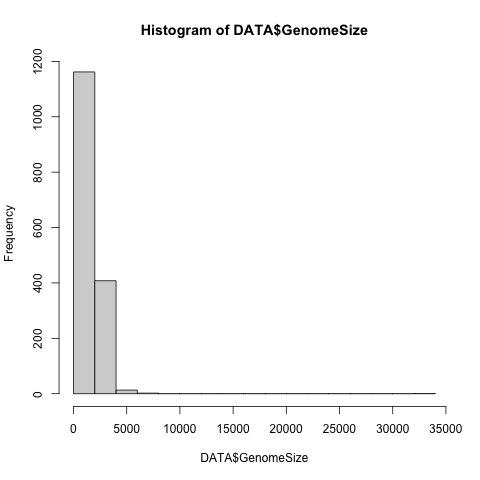
\includegraphics{images/genome_length_animals.png}
\caption{Showing animals genome length distribution}
\end{figure}

\hypertarget{further-analyses}{%
\subsection{Further analyses}\label{further-analyses}}

You can provide here the \texttt{bash} and \texttt{R} commands to
generate the genome sizes histograms for plants and bacteria (archea not
included). If you were able to perform and complete that task, you can
play with the data after that and provide box-plots by taxonomic group
showing the distribution of the genome sizes side-by-side.

\begin{Shaded}
\begin{Highlighting}[]
\CommentTok{# Your shell commands here}
\NormalTok{gawk }\StringTok{'BEGIN\{ FS=OFS="}\CharTok{\textbackslash{}t}\StringTok{"; \}}
\StringTok{$2 == "Eukaryota" && $3 == "Plants" \{}
\StringTok{print $0;}
\StringTok{\}'}\NormalTok{ stats}\OperatorTok{/}\NormalTok{genomes.tbl \textbackslash{}}
\OperatorTok{>}\StringTok{ }\NormalTok{stats}\OperatorTok{/}\NormalTok{genomes.plants_only.tbl}


\NormalTok{gawk }\StringTok{'BEGIN\{ FS=OFS="}\CharTok{\textbackslash{}t}\StringTok{"; \}}
\StringTok{$2 == "Bacteria" && ( $3 == "Terrabacteria group" || $3 == "Proteobacteria" || $3 == "unclassified" ) \{}
\StringTok{print $0;}
\StringTok{\}'}\NormalTok{ stats}\OperatorTok{/}\NormalTok{genomes.tbl \textbackslash{}}
\OperatorTok{>}\StringTok{ }\NormalTok{stats}\OperatorTok{/}\NormalTok{genomes.bacteria_only.tbl}
\end{Highlighting}
\end{Shaded}

\texttt{\{.r\}\ plants\ \textless{}-\ read.table("stats/genomes.plants\_only.tbl",\ \ \ \ \ \ \ \ \ \ \ \ \ \ \ \ \ \ \ \ \ header=FALSE,\ comment.char=\textquotesingle{}\#\textquotesingle{},\ \ \ \ \ \ \ \ \ \ \ \ \ \ \ \ \ \ \ \ \ col.names=c("SpeciesName","Superkingdom","TaxonGroup",\ \ \ \ \ \ \ \ \ \ \ \ \ \ \ \ \ \ \ \ \ \ \ \ \ \ \ \ \ \ \ \ \ "GenomeSize","ChromNum"),\ sep\ =\ \textquotesingle{}\textbackslash{}t\textquotesingle{});\ bacteria\ \textless{}-\ read.table("stats/genomes.bacteria.tbl",\ \ \ \ \ \ \ \ \ \ \ \ \ \ \ \ \ \ \ \ \ header=FALSE,\ comment.char=\textquotesingle{}\#\textquotesingle{},\ \ \ \ \ \ \ \ \ \ \ \ \ \ \ \ \ \ \ \ \ col.names=c("SpeciesName","Superkingdom","TaxonGroup",}
``GenomeSize'',``ChromNum''), sep = `\t');

\begin{Shaded}
\begin{Highlighting}[]
\CommentTok{#png(file = "images/plants.png")}
\KeywordTok{ggplot}\NormalTok{(plants, }\KeywordTok{aes}\NormalTok{(GenomeSize, }\DataTypeTok{fill =}\NormalTok{ TaxonGroup)) }\OperatorTok{+}\StringTok{ }\KeywordTok{geom_histogram}\NormalTok{(}\KeywordTok{aes}\NormalTok{(}\DataTypeTok{y =} \KeywordTok{stat}\NormalTok{(count) ), }\DataTypeTok{bins =} \DecValTok{8}\NormalTok{, }\DataTypeTok{show.legend =} \OtherTok{TRUE}\NormalTok{)}
\CommentTok{#dev.off()}
\end{Highlighting}
\end{Shaded}

\begin{figure}
\centering
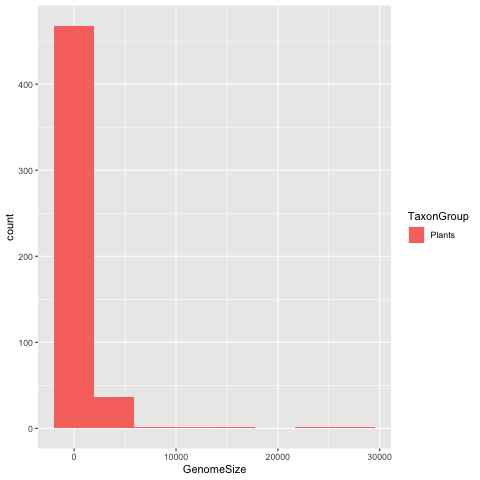
\includegraphics{images/plants.png}
\caption{Showing plants genome length distribution}
\end{figure}

\begin{Shaded}
\begin{Highlighting}[]
\CommentTok{#png(file = "images/bacteria.png")}
\KeywordTok{ggplot}\NormalTok{(bacteria, }\KeywordTok{aes}\NormalTok{(GenomeSize, }\DataTypeTok{fill=}\NormalTok{ TaxonGroup)) }\OperatorTok{+}\KeywordTok{geom_histogram}\NormalTok{(}\KeywordTok{aes}\NormalTok{(}\DataTypeTok{y =} \KeywordTok{stat}\NormalTok{(count) ), }\DataTypeTok{bins =} \DecValTok{8}\NormalTok{, }\DataTypeTok{show.legend =} \OtherTok{TRUE}\NormalTok{) }\OperatorTok{+}\StringTok{ }\KeywordTok{theme}\NormalTok{(}\DataTypeTok{legend.title =} \KeywordTok{element_text}\NormalTok{(}\DataTypeTok{size =} \DecValTok{3}\NormalTok{),}
               \DataTypeTok{legend.text =} \KeywordTok{element_text}\NormalTok{(}\DataTypeTok{size =} \DecValTok{3}\NormalTok{))}
\CommentTok{#dev.off()}
\end{Highlighting}
\end{Shaded}

\begin{figure}
\centering
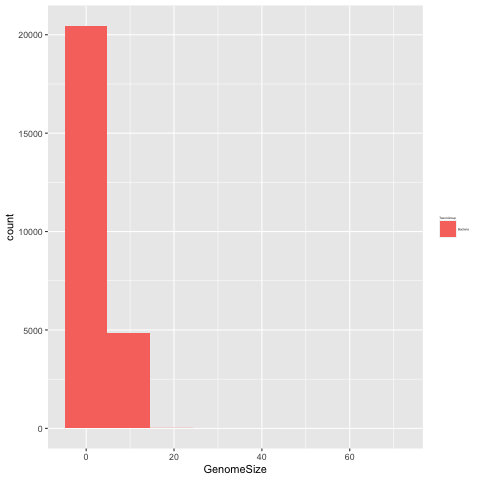
\includegraphics{images/bacteria.png}
\caption{Showing bacteria genome length distribution}
\end{figure}

\begin{Shaded}
\begin{Highlighting}[]
\NormalTok{bacteria}\OperatorTok{$}\NormalTok{TaxonGroup <-}\StringTok{ "Bacteria"}
\NormalTok{merge <-}\StringTok{ }\KeywordTok{do.call}\NormalTok{(rbind, }\KeywordTok{list}\NormalTok{(DATA,plants, bacteria))}
\CommentTok{#png(file = "images/merge.png")}
\KeywordTok{boxplot}\NormalTok{(merge}\OperatorTok{$}\NormalTok{GenomeSize}\OperatorTok{~}\NormalTok{merge}\OperatorTok{$}\NormalTok{TaxonGroup, }\DataTypeTok{xlab =} \StringTok{"Taxonomical Group"}\NormalTok{, }\DataTypeTok{ylab =} \StringTok{'Genome size'}\NormalTok{, }\DataTypeTok{col =} \KeywordTok{c}\NormalTok{(}\StringTok{'blue'}\NormalTok{,}\StringTok{'green'}\NormalTok{,}\StringTok{'red'}\NormalTok{))}
\CommentTok{#dev.off()}
\end{Highlighting}
\end{Shaded}

\begin{figure}
\centering
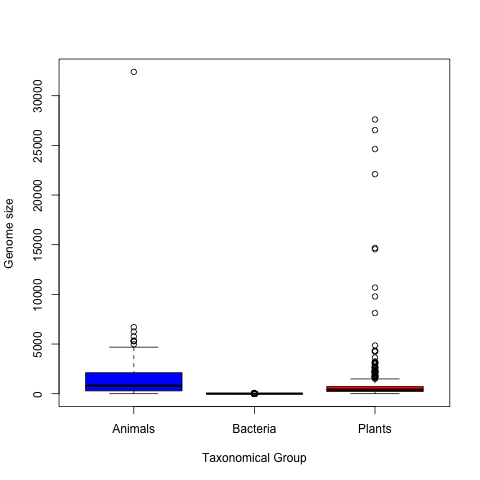
\includegraphics{images/merge.png}
\caption{Showing plants animals and bacteria genome length distribution}
\end{figure}

\hypertarget{discussion}{%
\section{Discussion}\label{discussion}}

\label{sec:discussion}

\textbf{IMPORTANT} Discuss your results here (around 300 words). And
remember to include in the Appendices section (see page
\pageref{sec:appendices}), any extra script you wrote from this exercise
\texttt{bin} folder using the \texttt{loadfile} macro.

:: \textbf{YOUR DISCUSSION OF RESULTS HERE} ::

Firstly, we can start talking about the boxplot comparing animals,
plants, and bacteria. We can state that in general, the more complex the
organism is the more tend to have a bigger genome size. The distribution
for plants and animals is more or less the same arround 8000 mbp, while
bacteria is smaller 15 mbp. Also, we can see that there are more
outliers for plants and animals than bacteria.

From the evolution, we know the complexity of the animals as organism.
Other organisms, like bacteria, can have more than one copy of its
genome and use it in different ways (more variability).

In prokaryotes (bacteria in our case), in general we can state that
there exist a linear relationship between genome size and the number of
genes. However, in eukaryotes we cannot say the same, there is no
correlation between the complexity of an organism and its genome, and it
is called as the C-value paradox.

References:

\begin{itemize}
\tightlist
\item
  The size of the genome and the complexity of living beings: A. Latorre
  and F. J. Silva:
  https://metode.org/issues/monographs/the-size-of-the-genome-and-the-complexity-of-living-beings.html\#:\textasciitilde{}:text=The\%20genome\%20of\%20an\%20organism,including\%20genes\%20and\%20intergenic\%20regions.\&text=However\%2C\%20in\%20eukaryotes\%20there\%20is,as\%20the\%20C\%2Dvalue\%20paradox.
\end{itemize}

\clearpage

\hypertarget{appendices}{%
\section{Appendices}\label{appendices}}

\label{sec:appendices}

\hypertarget{software}{%
\subsection{Software}\label{software}}

We have used the following versions:

\begin{Shaded}
\begin{Highlighting}[]
\FunctionTok{uname}\NormalTok{ -a}
\CommentTok{# Linux cocoon 4.19.0-4-amd64 #1 SMP Debian 4.19.28-2 (2019-03-15) x86_64 GNU/Linux}

\ExtensionTok{R}\NormalTok{ --version}
\CommentTok{# R version 3.5.2 (2018-12-20) -- "Eggshell Igloo"}
\CommentTok{# Copyright (C) 2018 The R Foundation for Statistical Computing}
\CommentTok{# Platform: x86_64-pc-linux-gnu (64-bit)}
\end{Highlighting}
\end{Shaded}

\hypertarget{supplementary-files}{%
\subsection{Supplementary files}\label{supplementary-files}}

\label{sec:supplfiles}

\hypertarget{project-specific-scripts}{%
\subsubsection{Project specific
scripts}\label{project-specific-scripts}}

\loadfile{an\_script\_example.pl}{bin/an_script_example.pl}{prg:scriptexamplePERL}

\hypertarget{shell-global-vars-and-settings-for-this-project}{%
\subsubsection{Shell global vars and settings for this
project}\label{shell-global-vars-and-settings-for-this-project}}

\loadfile{projectvars.sh}{projectvars.sh}{prg:projectvarsBASH}

\hypertarget{about-this-document}{%
\subsection{About this document}\label{about-this-document}}

This document was be compiled into a PDF using \texttt{pandoc} (see
\texttt{projectvars.sh} from previous subsection) and some
\texttt{LaTeX} packages installed in this linux system.
\texttt{synaptic}, \texttt{apt-get} or \texttt{aptitude} can be used to
retrieve and install those tools from linux repositories. As the
\texttt{raw\_tex} extension has been provided to the
\texttt{markdown\_github} and \texttt{tex\_math\_dollars} formats, now
this document supports inline \LaTeX~and inline formulas!

You can get further information from the following links about the
\href{http://daringfireball.net/projects/markdown/syntax\#link}{Mark
Down syntax}, as well as from the manual pages (just type
\texttt{man\ pandoc} and/or \texttt{man\ pandoc\_markdown}).


\end{document}
